\documentclass[]{article}
\usepackage[utf8]{inputenc}
\usepackage[T1]{fontenc}
\usepackage[total={11in,8.5in},portrait,left=1in,right=1in,top=1.5in]{geometry}
\usepackage{amsmath}
\usepackage{amsfonts}
\usepackage{textgreek}
\usepackage{graphicx}
\usepackage{hyperref}
\usepackage{doi}
\begin{document}
\title{BMI 203 Final Project}
\author{Garrett Wong}
\date{15 March 2019}
\maketitle

Code is at \url{https://github.com/garrett-wong/BMI203_FP}.

\section[2]{RAP1}

\subsection{Describe the machine learning approach in detail.}

I encoded the sequence data using a 1-hot method with a set of 3 binary dummy variables per base, indicating whether it is a ``C'', ``G'', or ``T'', respectively. (If none, it's an ``A''). These variables were flattened:

\[ [C_0, G_0, T_0, C_1, G_1, T_1, \ldots, C_n, G_n, T_n] \]

so, for example, the sequence ``ATG'' would be encoded $[0, 0, 0, 0, 0, 1, 0, 1, 0]$. This encoding allows bias and three weights to encode four independent parameters for each of the three bases' effect at each position.

I train a logistic regression classifier on these inputs. I perform L2-regularized logistic regression in order to penalize high coefficients and avoid overfitting.

I use a modified bagging technique. In each iteration, I fit the classifier to a same-sized bootstrap sample of the true positive sequences. In each of these samples $\approx \frac{1}{e}$ of the true positive sequences are not present. Averaging across these models fit to only part of the true positive data reduces variation and helps avoid overfitting.

\subsection{How was your training regime designed so as to prevent the negative training datafrom overwhelming the positive training data?}

Each time I fit the model, I draw a new dataset of negatives that is the same size as the set of positives, where each is a length 17 subset of one of the negative FASTA strings that doesn't match any of the true positives.

Because I feed the model the same set of positives and negatives, it doesn't become overwhelmed by the negatives. By feeding different negatives each time and averaging, I ensure that the model doesn't learn features specific to any given sample of negatives, forcing it to 
learn features of the positives instead.

\subsection{What was your stop criterion for convergence in your learned parameters? How did you decide this?}

The logistic regression model is solved once instead of being iteratively updated. However, somewhat analogously, I had to choose a number of bagging models to average. In order to determine if I was averaging enough models, I determined the summed distances between the probabilities of "True" labels given by the model and the 1 or 0 labels on a held-out $1/10$ of the data when averaging successive numbers of models. 

\vspace{1em}
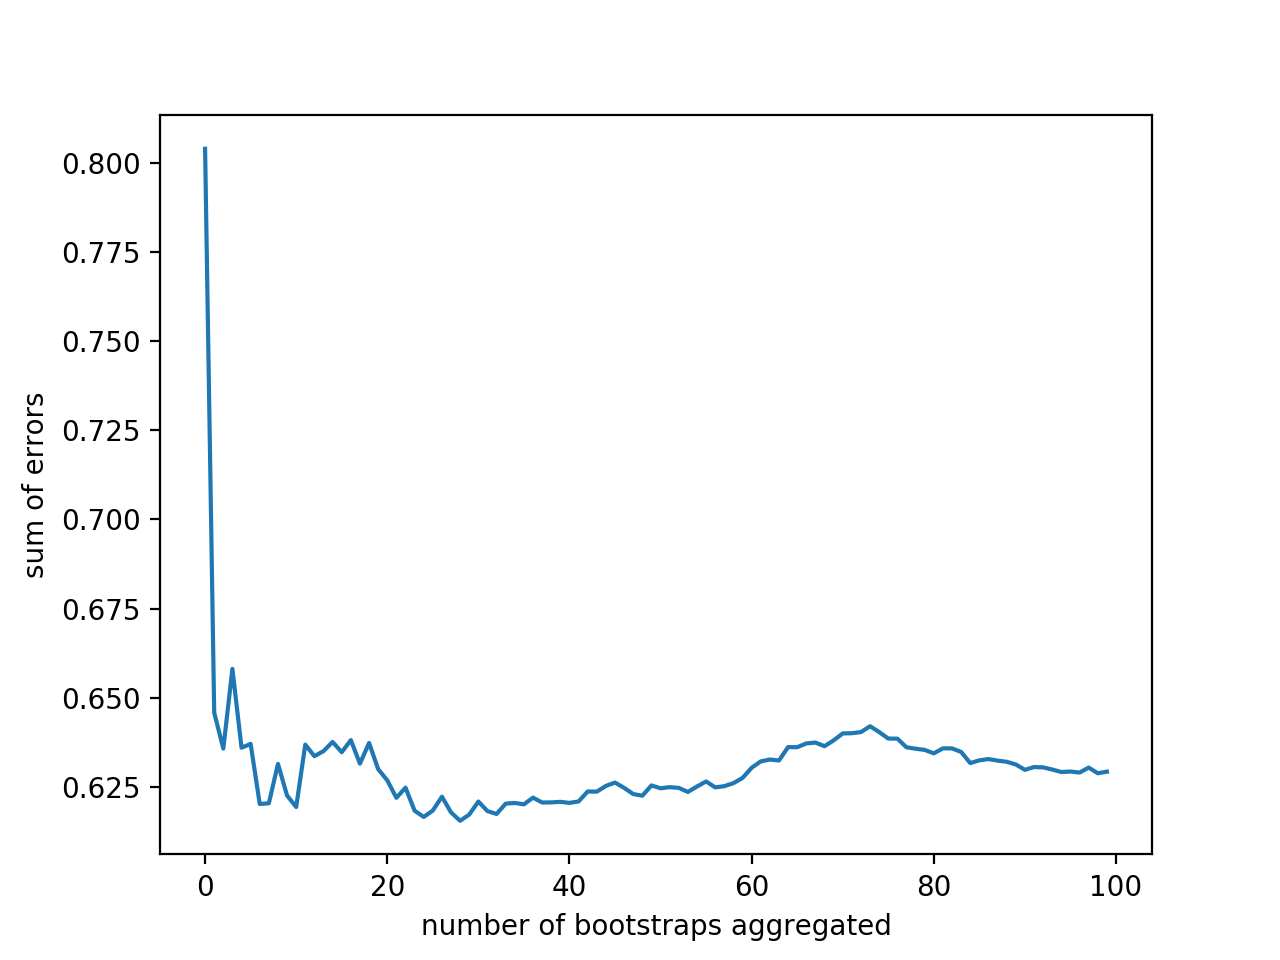
\includegraphics[width=0.5\textwidth]{numBaggingIterations.png}
\vspace{1em}

We can see that the variation between sums of errors for larger averages drops quickly as the number of models being averaged increases, as we would expect. 100 models is plenty, and still runs very quickly.

\subsection{Describe how you set up your experiment to measure your system's performance.}

In order to assess my model's performance, I performed something analogous to $k$-fold stratified cross validation with $k=8$. I divide my true positive data into $k$ sets and each time train on all but $k$ and test on the remaining $k$. Each time I train and test, I include an balanced-sized new sample of true negative data as described above.

Finally, in case there is still overfitting, I hold out $1/10$ of the data before performing any cross-validation; after cross-validation, I test on this never-seen data.

To assess the performance of my model, I determine the accuracy of the model in the test data (the ($1/k$) sequences not used to train the model), as well as the accuracy in the held-out $1/10$.

\vspace{1em}
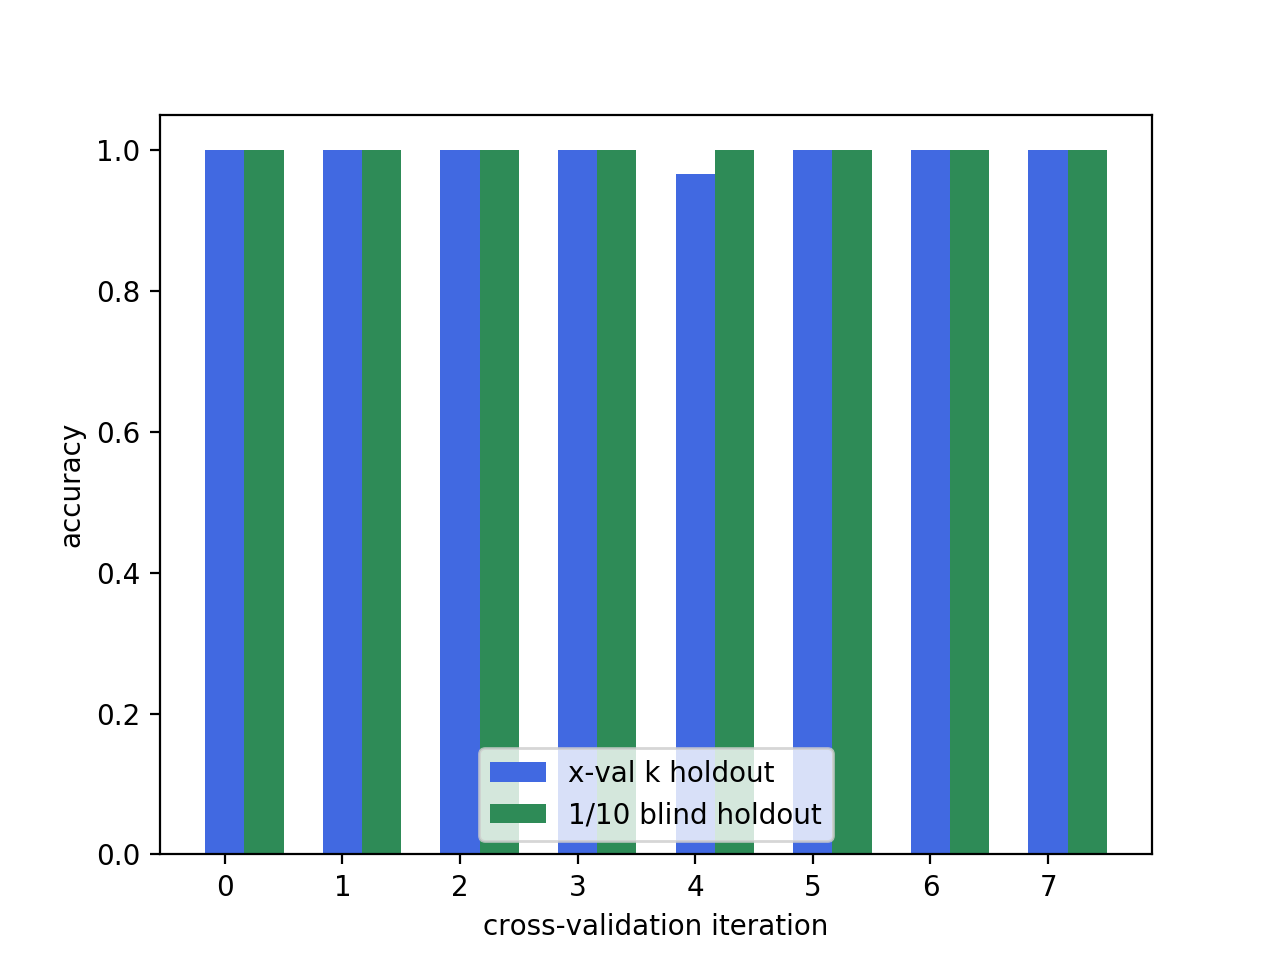
\includegraphics[width=0.5\textwidth]{xvalAccuracy.png}
\vspace{1em}

The accuracy is very high; with our small hold-out it's likely to perform with an accuracy of $> 1 - 1/14$ if given a new sample of true positive data and true negative data drawn from the same distributions.

\subsection{What set of learning parameters works the best? Please provide sample output from your system.}

I tried varying the norm and using the weaker L1 norm:

\vspace{1em}
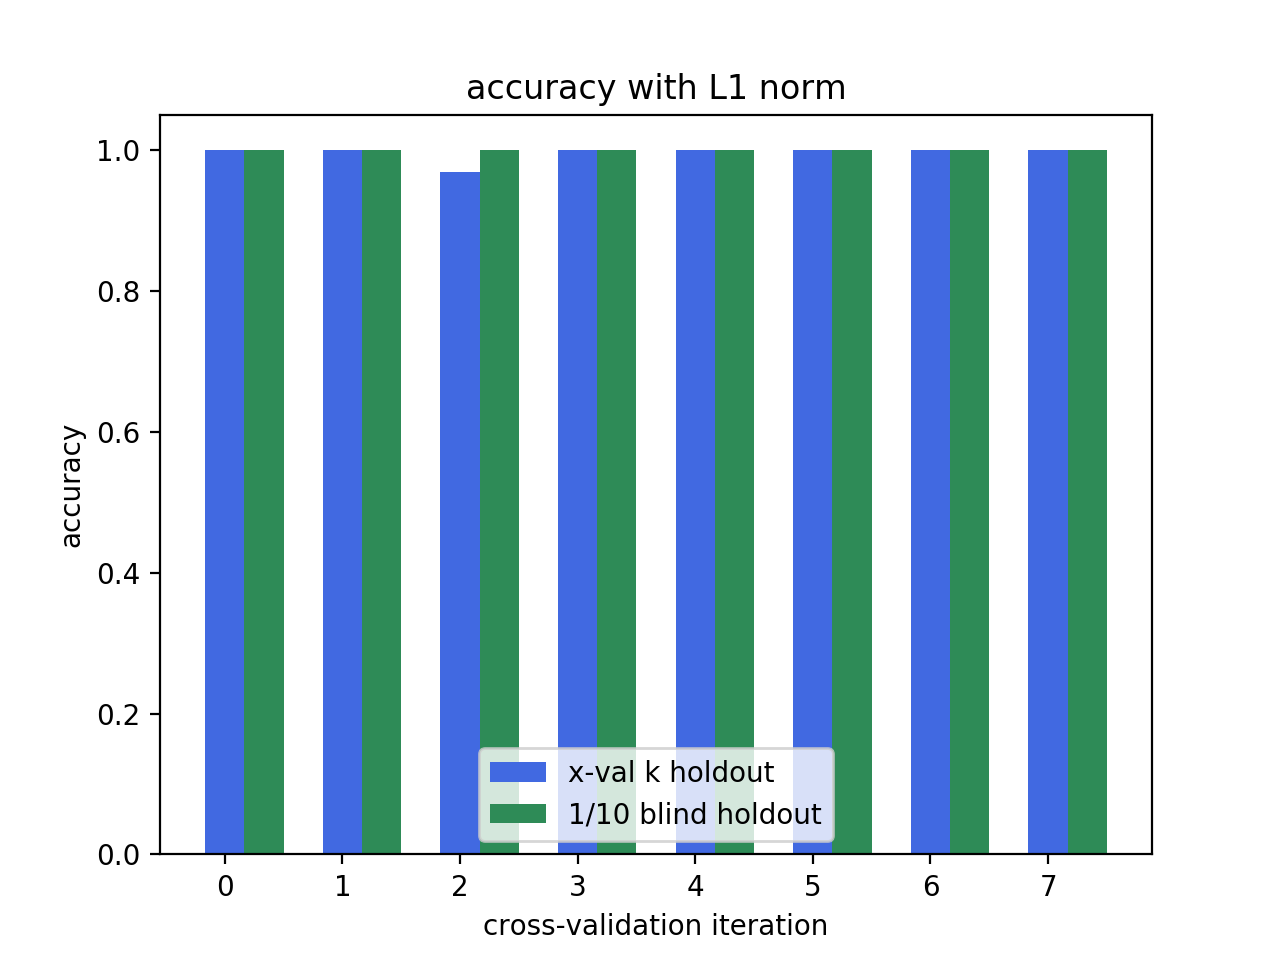
\includegraphics[width=0.5\textwidth]{xvalAccuracyL1.png}
\vspace{1em}

It did little to decrease the accuracy of the model, but I found that if I also decreased the regularization strength to $1/10000$, the non-regularized parameters started to lead to worse prediction in the test sets:

\vspace{1em}
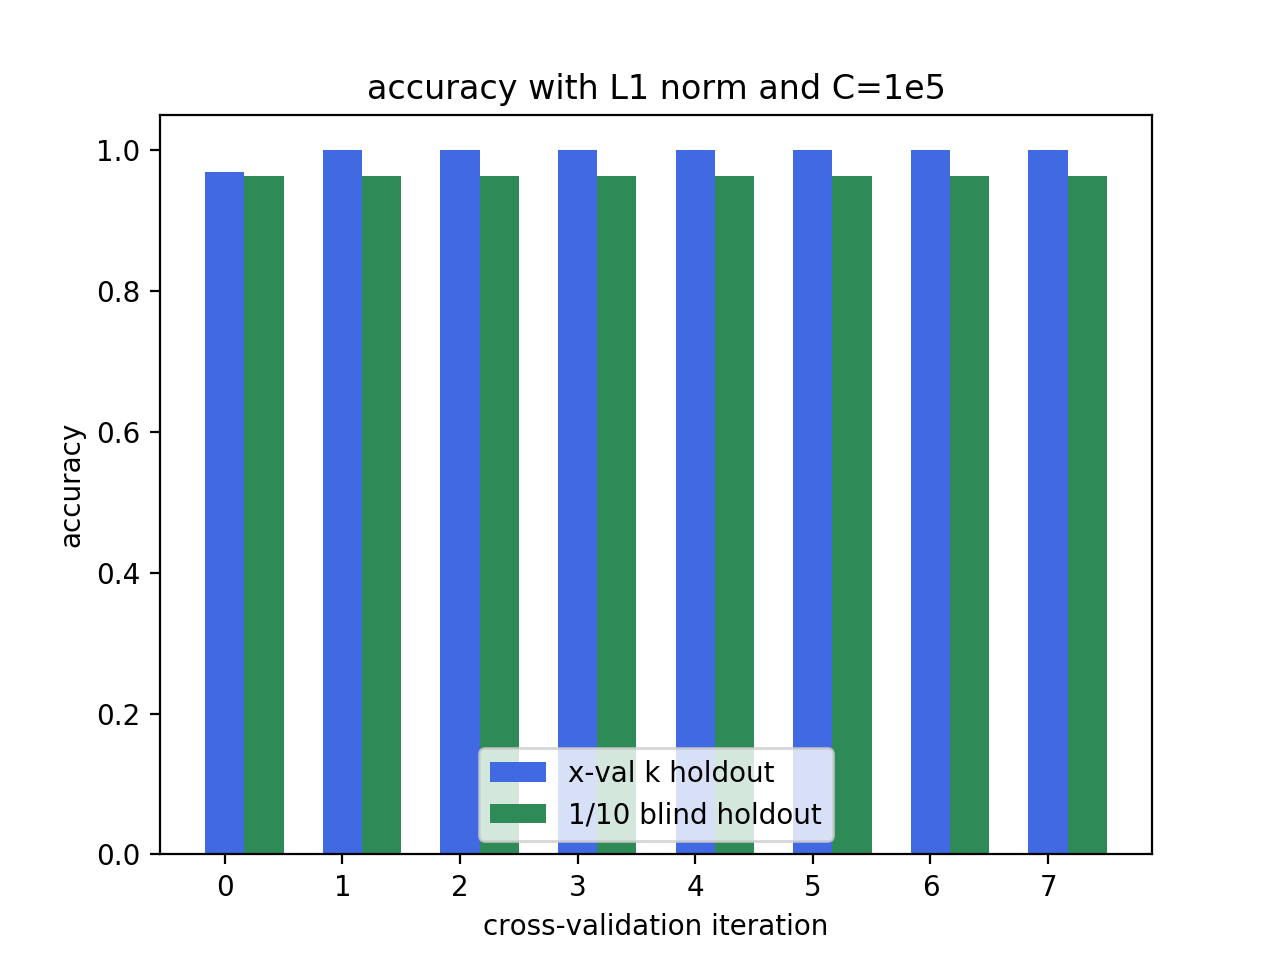
\includegraphics[width=0.5\textwidth]{xvalAccuracyL1c1e5.png}
\vspace{1em}

\subsection{What other parameters, if any, affect performance?}

Finally, I tried a different representation of input, as suggested in \doi{10.1101/186965}: ordinal, with A:0.25, C:0.5, G:0.75, and T:1. Even though this reduces the dimensionality of the input data, the accuracy is still surprisingly good.


\vspace{1em}
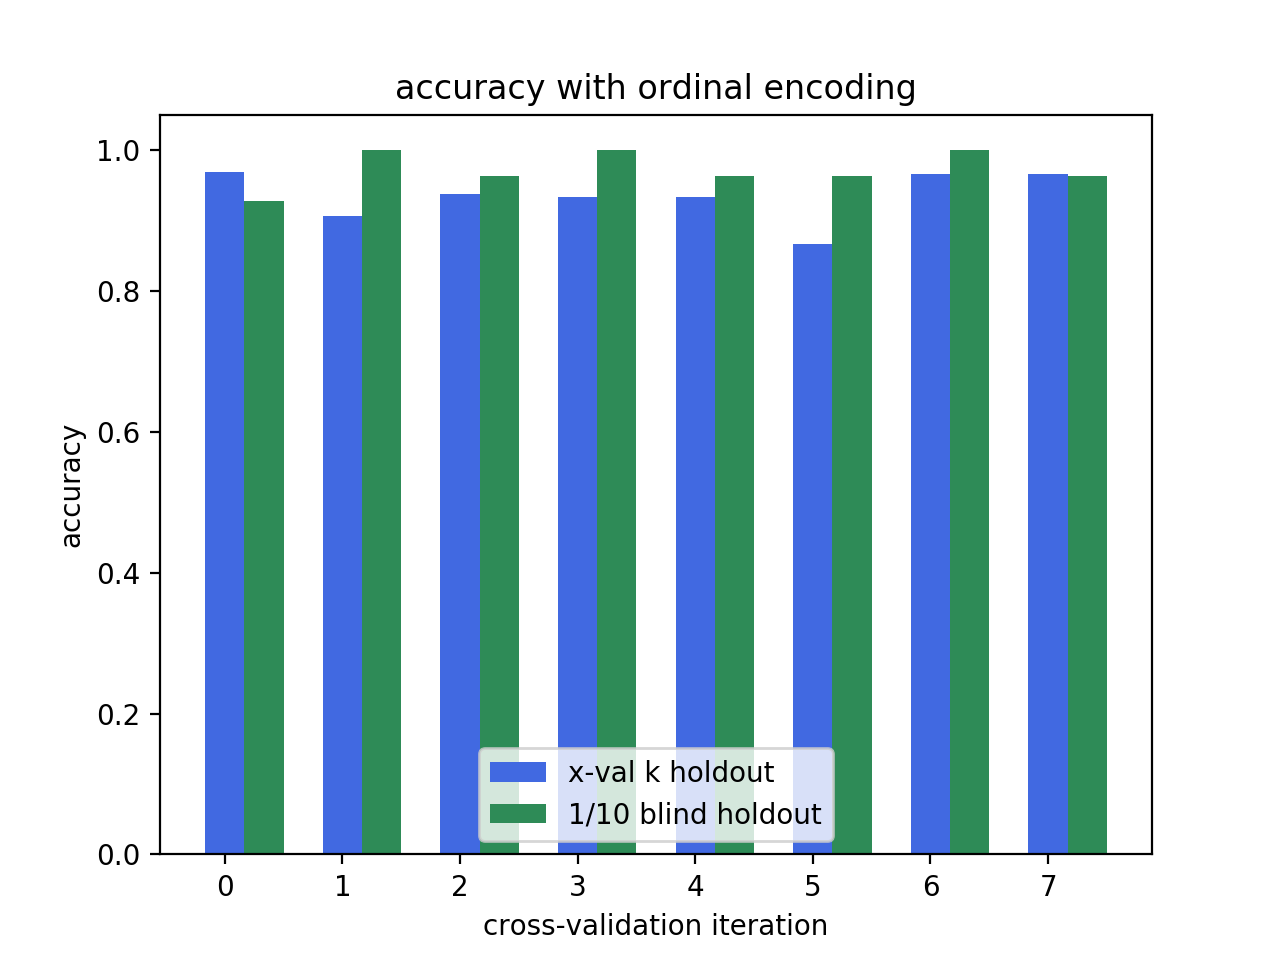
\includegraphics[width=0.5\textwidth]{xvalAccuracyOrdinal.png}
\vspace{1em}

\end{document}




